\documentclass[11pt]{scrartcl}
\usepackage[utf8]{inputenc} % Kodierung der Textdatei mit Sonderzeichen
\usepackage[ngerman]{babel} % Sprache fuer Inhaltsverzeichnis etc.
\usepackage{amssymb} % Mathematische Symbole
\usepackage{amsmath} % Mehr mathematische Konstrukte
\usepackage{graphicx} % Um Bilder einbinden zu koennen
\usepackage{float} % fuer \begin{figure}[H]
\usepackage{icomma} % laesst das Komma als Dezimaltrennzeichen interpretieren
\usepackage{fix-cm} % für die große Titelschrift
\usepackage[pdftex]{hyperref} % Hyperlinks im Dokument
\hypersetup{colorlinks=true, linkcolor=black, citecolor=black, filecolor=black, urlcolor=black, pdftitle={LED-Spektrometer - Projektpraktikum 09/10 Gruppe 5}}


\newcommand{\unit}[1]{\ensuremath{\,\mathrm{#1}}} % Einheiten schreiben sich immer aufrecht!
\newcommand{\degr}{\ensuremath{^\circ}}
\newcommand{\cel}{\ensuremath{\degr\mathrm{C}}}
\newcommand{\dif}{\ensuremath{\mathrm{d}}}
\newcommand{\pdif}[2]{\ensuremath{\frac{\partial#1}{\partial#2}}}
\newcommand{\ee}[1]{\ensuremath{\cdot 10^{#1}}}
\newcommand{\hypref}[2]{\hyperref[#2]{{#1}~\ref{#2}}}

\setlength{\parindent}{1em}
\setlength{\parskip}{0.5\baselineskip}


\title{Direkte Messung der Erdrotation - Gruppe 5 WS 09/10, Projektpraktikum der Uni Erlangen}
\date{07.12.2009 -- 15.01.2010}
\author{Michele Collodo, Andreas Glossner, Karl-Christoph G\"odel, Bastian Hacker, Maria Obst, Alexander Wagner, David Winnekens}



\begin{document}
\sloppy % laesst Latex nicht ueber den Rand rausschreiben
\thispagestyle{empty}
\large{Projektpraktikum WS 09/10}
\hfill
\raisebox{-1.4cm}{\includegraphics[width=5cm]{images/fau.pdf}}
\\[8\baselineskip]
\begin{center}
{\fontsize{36}{54}\textbf{Direkte Messung der Erdrotation}}
\\[2\baselineskip]
{\Large 07.12.2009 -- 15.01.2010}
\\[7\baselineskip]
{\huge\textbf{PPG 5}}
\\[0.5\baselineskip]
{\large\textbf{
Michele Collodo,
Andreas Glossner,\\
Karl-Christoph G\"odel,
Bastian Hacker,\\
Maria Obst,
Alexander Wagner,
David Winnekens}\\
Tutor: Xiaoyue Jin}
\vfill



\small{\url{http://pp.physik.uni-erlangen.de/groups/ws0910/ppg5/ppg5\_start.html}}
\end{center}
\newpage



\tableofcontents
\vfill



\begin{abstract}
Bla Abstract Bla
\end{abstract}
\newpage

\section{Einleitung}
Messung der Erdrotation - eines der \"altesten Experimente der Physik
\section{Grundprinzip - Tr\"agheitsmoment}

\begin{figure}[ht]
\begin{center}
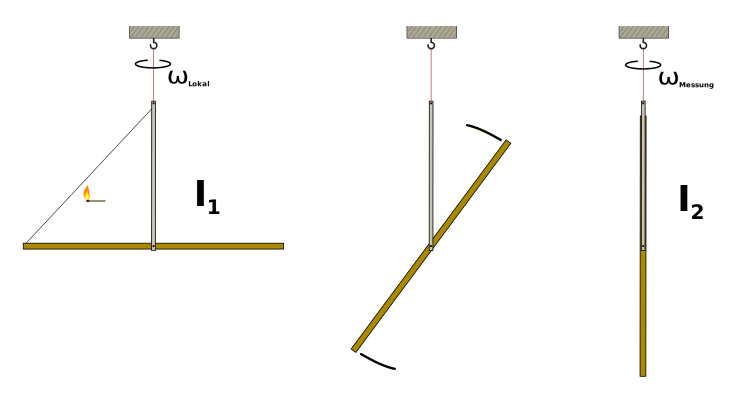
\includegraphics[width=0.8\textwidth]{images/prinzip.pdf}
\end{center}
\vspace{-1.5\baselineskip}
\caption{Schema des Bewegungsablaufs}
\label{prinzip}
\end{figure}

\subsection{Bau des Drehstabs}
\subsubsection{Material}
Magnetismus, Verwindung usw.
\subsubsection{Aufh\"angung}
Stabilisierung der Drehbewegung
\subsubsection{Klappmechanismus}
Zugmechanismus, Einrasten

\begin{figure}[ht]
\begin{center}
\includegraphics[width=0.8\textwidth]{images/stab-fertig.jpg}
\end{center}
\vspace{-1.5\baselineskip}
\caption{Der ausgelenkte Stab}
\label{stab-fertig}
\end{figure}

\subsection{Messungen}
\subsubsection{Berechnungen im Vorraus}
Tr\"agheitsmoment Rechnungen von Andi

\begin{figure}[ht]
\begin{center}
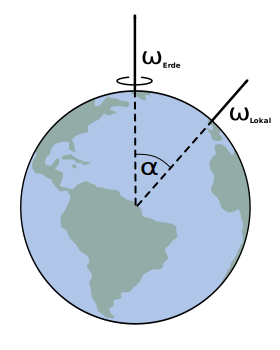
\includegraphics[width=0.2\textwidth]{images/welt.pdf}
\end{center}
\vspace{-1.5\baselineskip}
\caption{Position auf der Welt}
\label{Welt}
\end{figure}

\subsubsection{Auswertung der Messdaten}
Schrott ?? 

\subsection{Fazit}
Nicht alles funktioniert so, wie erwartet \dots $\rightarrow$ Warum?


\newpage
\section{Autorenverzeichnis}
\begin{tabular}{|l|l|}
\hline
\emph{Autor} & \emph{Kapitel}\\
\hline
Michele Collodo & \\
Andreas Glossner & \\
Karl-Christoph G\"odel & \\
Bastian Hacker & \\
Maria Obst & \\
Alexander Wagner & \\
David Winnekens &  \\
Wickie Pedia & Recherchen \\
\hline
\end{tabular}
\end{document}